\chapter{Convolutional Neural Networks}
\begin{figure}[H]
    \centering
    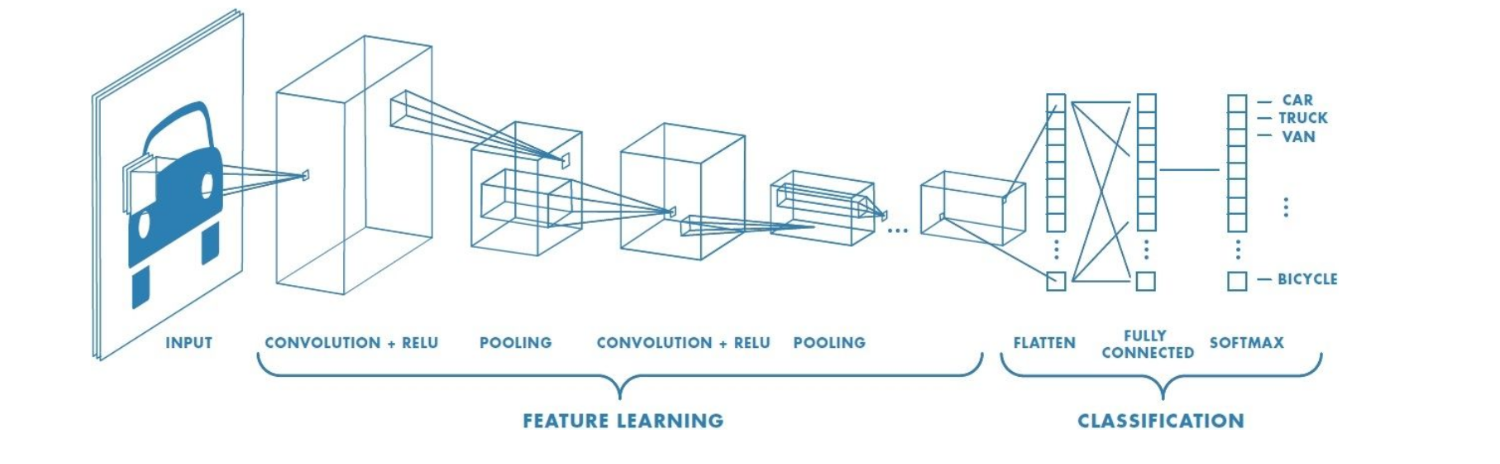
\includegraphics[width=0.75\linewidth]{img/CNN_diagram.png}
\end{figure}


\section{Introduction}

 CNNs are a specialised kind of neural network that are designed to process data that comes in the form of multiple arrays, such as colour images composed of 2D pixel arrays for each colour channel.

\section{CNN Architecture}

The architecture of a CNN is engineered to take advantage of the 2D structure of an input image, performing convolution on its input as form of feature extraction. This involves sliding filter matrices, or kernels, across the input data to produce feature maps that summarise the presence of detected features in the input.

Key components of CNNs include:

\begin{itemize}
    \item \textbf{Convolutional layers:} These layers apply a number of filters to the input. Each filter detects different features by performing a convolution operation.
    \item \textbf{Filters and Feature Maps:} Filters are small, learnable weights that convolve over the input to produce feature maps, representing detected features.
    \item \textbf{Strides:} The stride defines the step size the filters take during the convolution operation across the input.
    \item \textbf{Padding:} Padding can be added to the input volume to allow the filter to cover the border of the input, thereby adjusting the spatial size of the output volume.
    \item \textbf{Pooling layers:} These layers reduce the dimensions of the data by combining the outputs of neuron clusters at one layer into a single neuron in the next layer.
    \item \textbf{Fully Connected (FC) layers:} After several convolutional and pooling layers, the high-level reasoning in the neural network is done via fully connected layers. Neurons in a fully connected layer have full connections to all activations in the previous layer.
    \item \textbf{Loss layers:} At the end of the network, a loss layer defines how the network's predictions are compared to the true data labels for the purpose of learning during training.
\end{itemize}
\section{CNN Overview and Input Data}
\begin{itemize}
    \item \textbf{Neural Network Architecture Optimisation:} CNNs are optimised for k-D data structures like images, including RGB or hyperspectral images.
    \item \textbf{Tensor Representation:} An image is represented as a 4D tensor with dimensions corresponding to the number of samples, height, width, and color channels of the input data.
    \item \textbf{Local Correlation:} Due to the nature of images, neighbouring pixels are often correlated, and this spatial correlation is leveraged by CNNs to reduce the number of parameters and computational complexity.
\end{itemize}



Images are represented as 4D tensors in CNNs: (samples, height, width, channels).\\

\begin{commentbox}{What's a Tensor?}
    
A tensor is a mathematical object that can be thought of as a generalised form of matrices. A tensor can have multiple dimensions, often referred to as ``axes". Each dimension of a tensor can represent different aspects of the data. 

\begin{itemize}
    \item0D Tensor (Scalar): A single number. For example, 5 or -3.2.
    \item1D Tensor (Vector): An array of numbers. For example, [1, 2, 3].
    \item2D Tensor (Matrix): An array of arrays of numbers. For example, [[1, 2, 3], [4, 5, 6]].
    \item3D Tensor: An array of matrices. In image processing, a 3D tensor can represent a color image where there are three matrices corresponding to the Red, Green, and Blue (RGB) color channels. This would look like: 
    \[
    \begin{bmatrix}
        [100,0,230] & [255,255,0] & [12,70,123]\\
        [12,5,1] & [89,4,12] & [123,6,82]\\
        [0,0,0] & [255,255,255] & [204,211, 90]
    \end{bmatrix}
    \]
    \item4D Tensor: Used in CNNs to store a batch of images. Each `slice' of this 4D tensor is a 3D tensor representing one image.
\end{itemize}
\end{commentbox}

These dimensions correspond to the number of samples in a batch, the image height, the image width, and the number of colour channels.\\

Filter convolutions are performed as shown in the diagram below:
\begin{figure}[H]
    \centering
    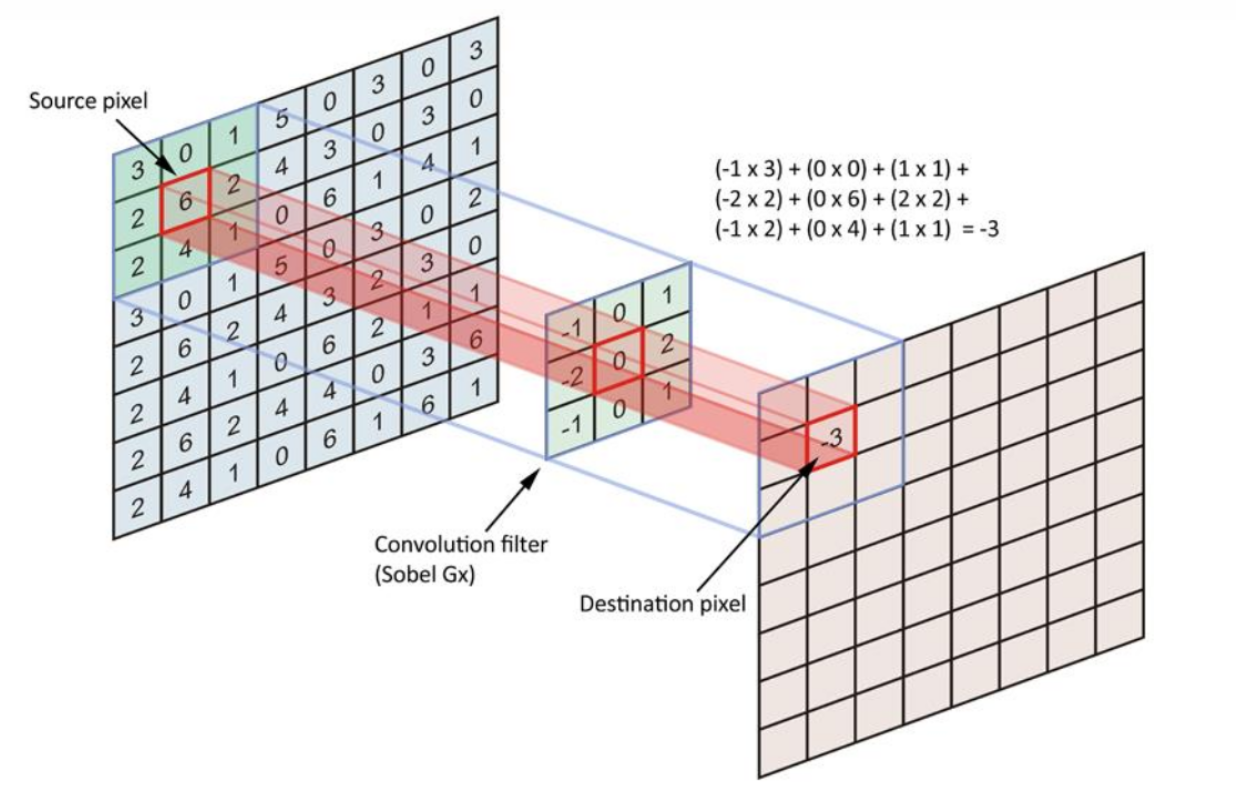
\includegraphics[width=0.75\linewidth]{img/CNN_filter.png}
    
    
\end{figure}

Now assume we have a \(30 \times 30 \times 3\) image. We reserve a 5-level filter for each pixel. Each filter has a  \(7 \times 7\) input. Spatially, we can arrange \(30 {\color{teal}+1}-7 = 24\)  filters across the x-axis so they receive a unique input, and the same for the y-axis. Each filter has \( 7 \times 7 \times 3\) parameters. As we have a depth of 5 levels, we multiply again. \\

\begin{figure}[H]
    \centering
    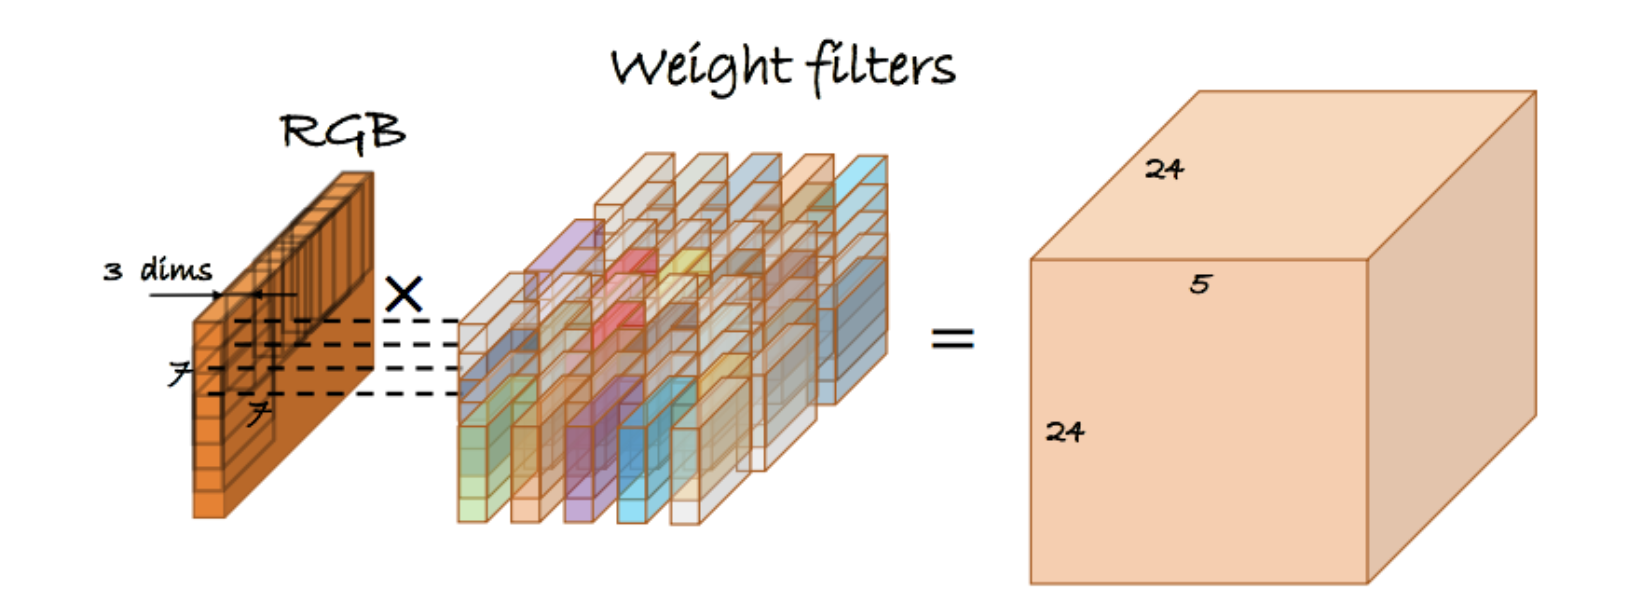
\includegraphics[width=0.75\linewidth]{img/cnn_1.png}
    
    
\end{figure}

The total number of parameters is:
\[
\underbrace{24}_{\text{x-axis}} \times \underbrace{24}_{\text{y-axis}} \times \underbrace{ 7 \times 7 \times 3}_{\text{filter parameters}} \times \underbrace{5}_{\text{filter depth}} = 423\text{k parameters}
\]

(To find out why we {\color{teal}+1}, try visualise this with a simpler example, like \(2 \times 2\) filters on a \(4 \times 4\) image.)

To which, we see the need for an excessive amount of parameters. If we had a \(256 \times 256\) image, we would need \(46 \times 10^6\) parameters.\\

We can do better by repeating filters as a sliding window. Now these filters are transient.

\begin{figure}[H]
    \centering
    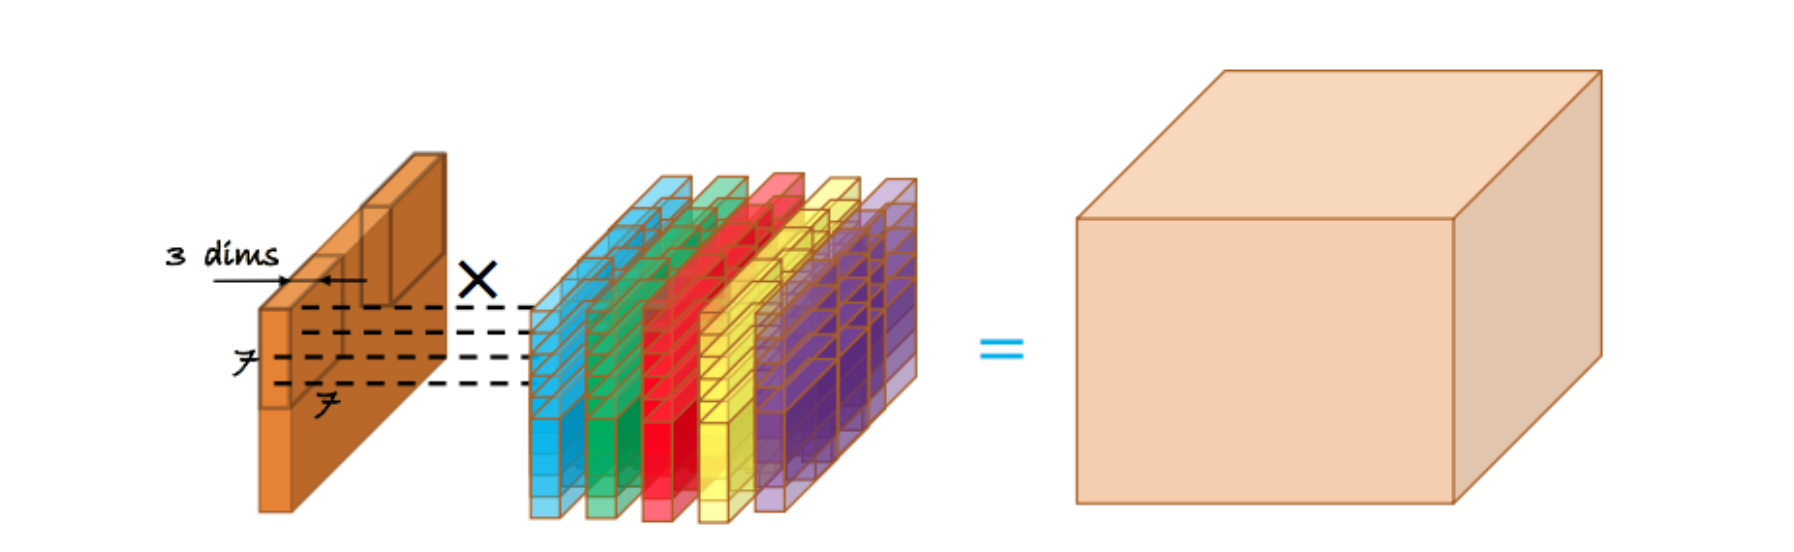
\includegraphics[width=0.75\linewidth]{img/cnn_2.png}
    
    
\end{figure}

The total number of parameters is now:
\[
 \underbrace{ 7 \times 7 \times 3}_{\text{filter parameters}} \times \underbrace{5}_{\text{filter depth}} = 735\text{ parameters}
\]

More generally, the output size, is computed by:

\[
    H_o = H_i - K + 1
\]

Where \(H_o\) is the output height, \(H_i\) is the input height, K is the kernel(filter) size.


\section{Convolution}

Convolution is a mathematical operation that is central to convolutional neural networks. It serves as a tool for feature extraction and is used to process data by applying a filter or kernel.

\subsection{Convolution in Continuous Space}

The convolution operator is defined in the continuous space as an integral transform. It is given by the integral of the product of two functions after one is reversed and shifted:

\[
(f * w)(t) = \int_{-\infty}^{+\infty} f(\tau) w(t - \tau) d\tau
\]

This operation can be understood as a weighted average of the function \( f \) across time or space, using the weighting function \( w \), which is the filter or kernel. The result is a new function that expresses how the shape of one function is modified by the other.

\subsection{Discrete Convolution}

In digital applications where signals are represented discretely, convolution is implemented as a sum:

\[
(f * w)(t) = \sum_{\tau=-\infty}^{+\infty} f(\tau) w(t - \tau)
\]

In practice, since signals and kernels are finite, the bounds of summation are limited to the extent of the defined functions.

\subsection{1D and 2D Discrete Convolution}

For a one-dimensional discrete signal, the convolution is a sum over the product of two discrete functions, one of which is flipped and shifted:

\[
(x * F)(i) = \sum_m x(m) F(i - m)
\]

In two dimensions, which is the common case for image processing, the convolution is a sum over both dimensions:

\[
(x * F)(i, j) = \sum_m \sum_n x(m, n) F(i - m, j - n)
\]

Alternatively, if we consider \( x \) as the input and \( F \) as the kernel or filter, the 2D convolution can also be expressed as:

\[
(x * F)(i, j) = \sum_m \sum_n x(i + m, j + n) F(m, n)
\]

The choice of the convolution expression can depend on the indexing convention, but the core concept remains the same. Different convolutions can create feature maps that highlight important features such as edges, textures, and shapes that are essential for understanding the content of the image.

\begin{figure}[H]
    \centering
    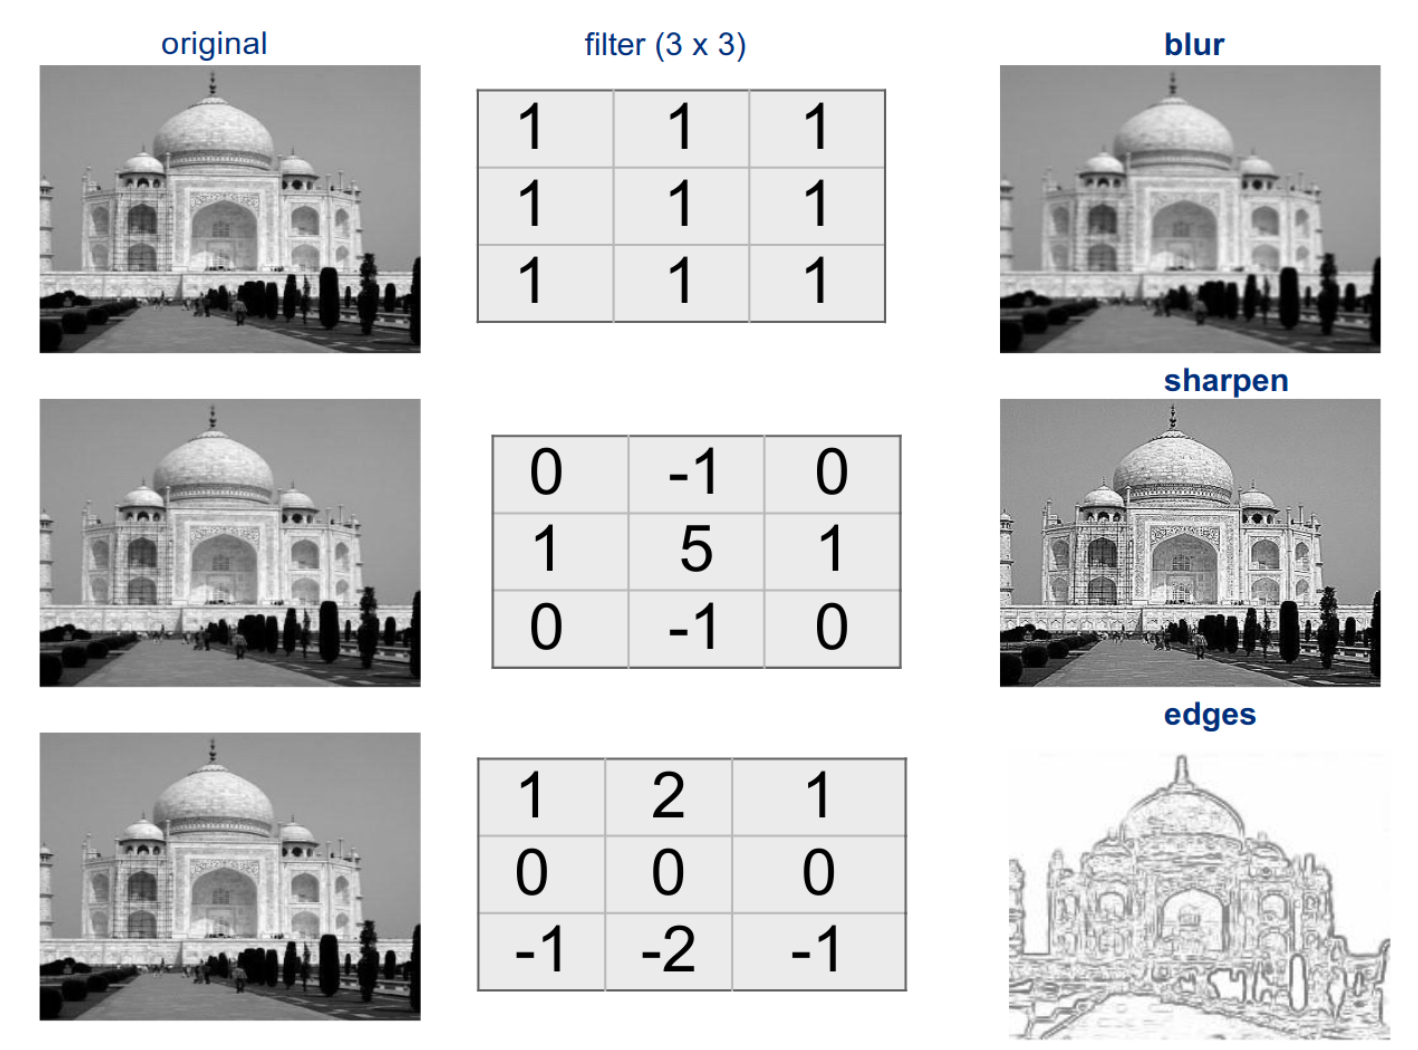
\includegraphics[width=0.75\linewidth]{img/kernels.png}
    
\end{figure}


\begin{definitionbox}{Convolutional Layer}

The convolutional layer is the core building block of a Convolutional Neural Network (CNN). It applies a set of learnable filters to the input data to create feature maps that capture spatial hierarchies of features.

\subsection{Convolution Operation}

Each filter in a convolutional layer has a receptive field, which is the size of the filter or kernel. This field determines the extent of the area in the input data over which the filter is applied.

\begin{itemize}
    \item The output of a filter, the result of a convolution, is a feature map.
    \item A layer can be formed from several channels. Typically there are many filters and feature maps for the same input, with an RGB image having three channels.
    \item Thus, filters or kernels are multi-dimensional tensors as well.
\end{itemize}

The convolution operation is applied across all channels of the input:

\[
\sum_{m}\sum_{n}\sum_{c} x(i + m, j + n, c) F(m, n, c)
\]

where \( x \) represents the input data, \( F \) represents the filter, \( i \) and \( j \) are spatial indices, and \( c \) is the index over the channels.

\subsection{Bias and Activation}

After the convolution operation, a bias term is usually added to the resulting feature map. This bias term is shared across the entire feature map. The final step in the convolutional layer is the application of an activation function to introduce non-linearity into the model:

\[
\theta\left(\sum_{m}\sum_{n}\sum_{c} x(i + m, j + n, c) F(m, n, c) + b\right)
\]

where \( b \) represents the shared bias. \\

The convolutional layers are stacked together, with each layer learning increasingly complex features. The combination of convolution, bias addition, and non-linear activation forms the fundamental components of feature learning in CNNs.

\end{definitionbox}

\section{Strides}
Strides refer to the step of the shift when applying the filter. The most use stride is \(1 \times 1\) stride that shifts a filter by one pixel at a time.\\

Note that for a \( 2 \times 2\) stride, each pixel is only ran through a filter once, so one path is skipped both horizontally and vertically. 

\begin{figure}[H]
    \centering
    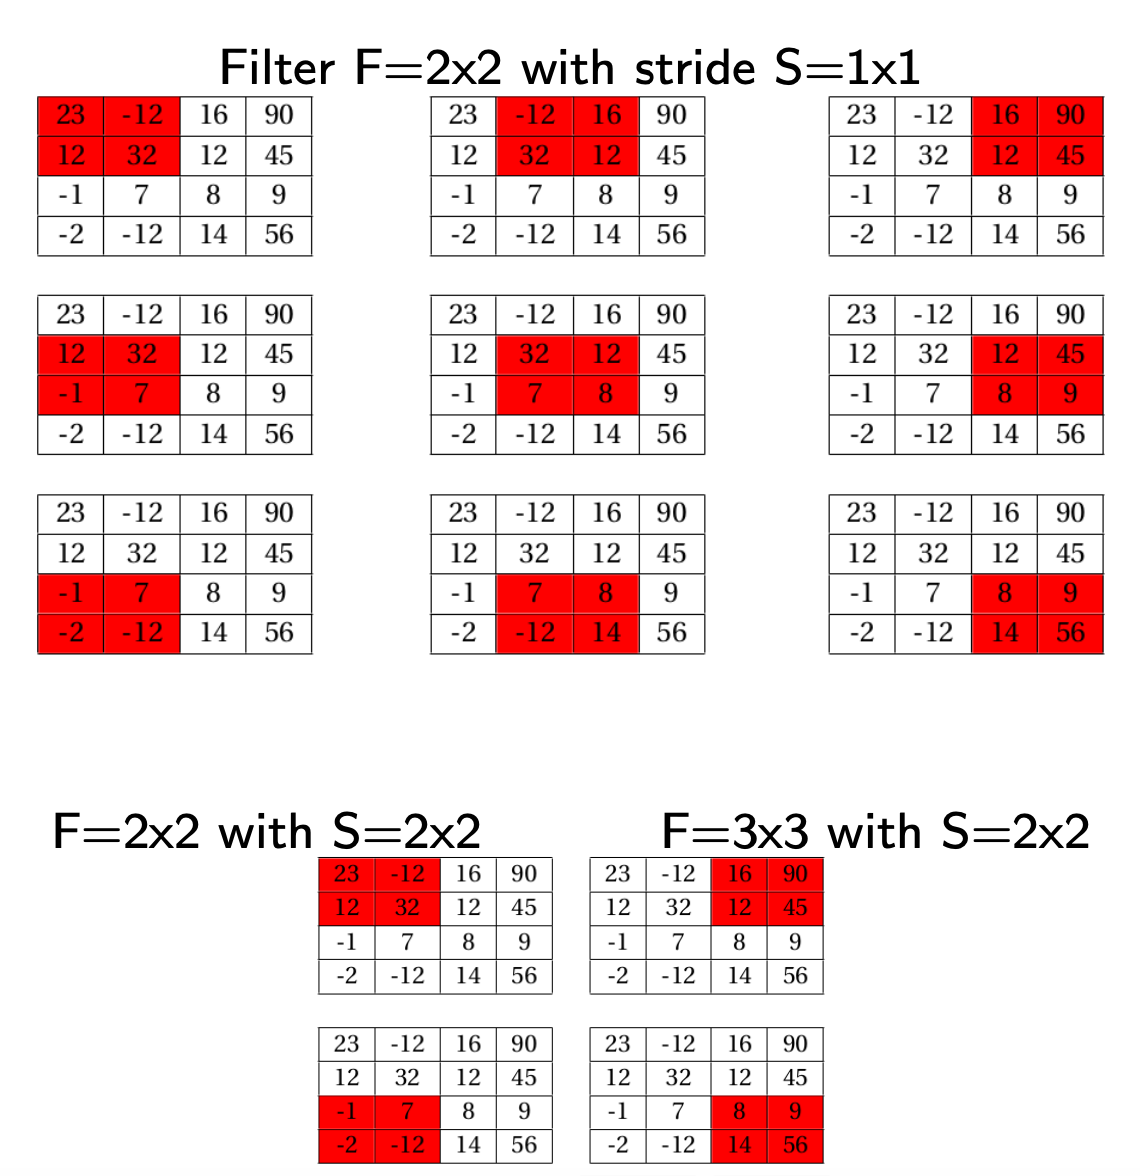
\includegraphics[width=0.75\linewidth]{img/strides.png}
    \caption{Different illustrations of strides for a given image input}
    
\end{figure}

\section{Padding}
Notice that applying the kernel map to the input feature map will result in a smaller output feature map size. This also results in information loss near the borders of the image input map. Some of the naming follows  the \texttt{tensorflow} library.

\begin{itemize}
    \item Note that $K$ refers to the size of the kernel(filter).
    \item VALID padding leaves the input feature map unchanged
    \item SAME padding adds $P=K-1$ zeroes to the input to constrain the output size to be the same for the unit strides. For odd-sized kernels, $P=\lfloor K/2\rfloor $ zeroes are added. So the heights of the input and output are the same, $H_o = H_i$
    \item Full padding adds $P=2(K-1)$ zeroes to the input, with $K-1$ zeroes on both sides. The output height $H_o$ is equal to the input height $H_i$ plus $2(K-1)$. So $H_o = H_i + 2(k-1)$

    
\end{itemize}

The output size for a given padding amount is computed by:

\[
H_o = H_i - K + 2P + 1
\]

Where \(P\) is the padding value.\\

When considering strides, the formula is:

\[
H_o = \frac{H_i - K + 2P}{S} + 1
\]

Where \(S\) is the stride value.

\begin{figure}[H]
    \centering
    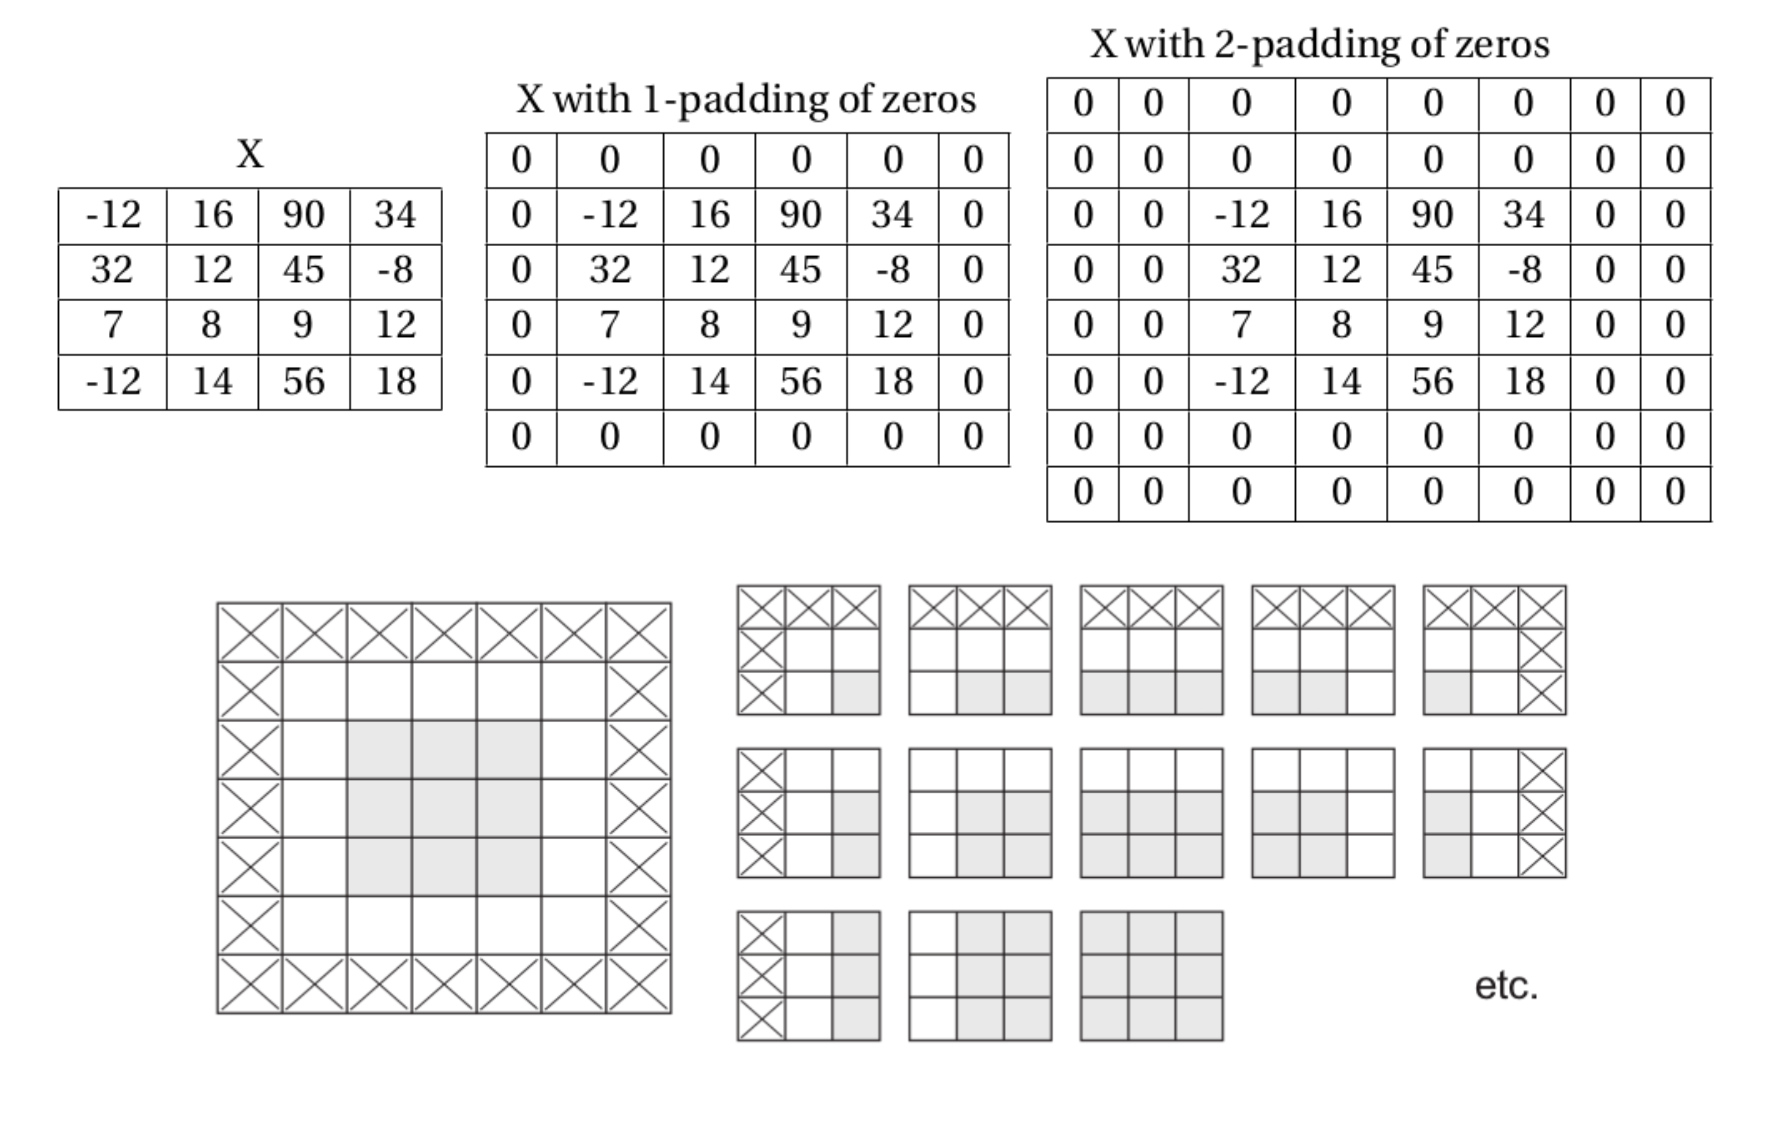
\includegraphics[width=0.75\linewidth]{img/padding.png}
    \caption{Visualisation of different padding levels. Note that to achieve SAME padding for the unlabelled example below, there must be a padding of 2 zeroes thick.}
    
\end{figure}

\section{CNN Properties}
\subsection{CNN Properties Overview}

\begin{itemize}
    \item \textbf{Sparse Connectivity:} Neurons in a CNN layer are connected only to a small region of the layer before it. A small visual field (receptive field) provides enough local information for feature extraction.
    \item \textbf{Shared Weights:} CNNs use the same filter (set of weights) for each position in the input volume, greatly reduces the number of parameters and complexity.
    \item \textbf{Translational Invariance:} Once a feature is learned, the network can recognise it in any other location of the input, although cannot handle rotation or scaling of the feature.
    \item \textbf{Local Correlation:} CNNs take advantage of the fact that nearby pixels in an image are more likely to be correlated, forming recognisable patterns.
    \item \textbf{Flexibility in Input Size:} CNNs can handle inputs of varying sizes for all sizes of images
    \item \textbf{Hierarchical Structure:} The layers of a CNN have the capability to act as a sequence of increasingly complex pattern detectors. Early layers may detect simple edges or textures, while deeper layers can detect more complex structures, such as parts of objects, and even more comprehensive layers can recognise whole objects or scenes.

\begin{figure}[H]
    \centering
    \begin{subfigure}[b]{0.45\linewidth}
        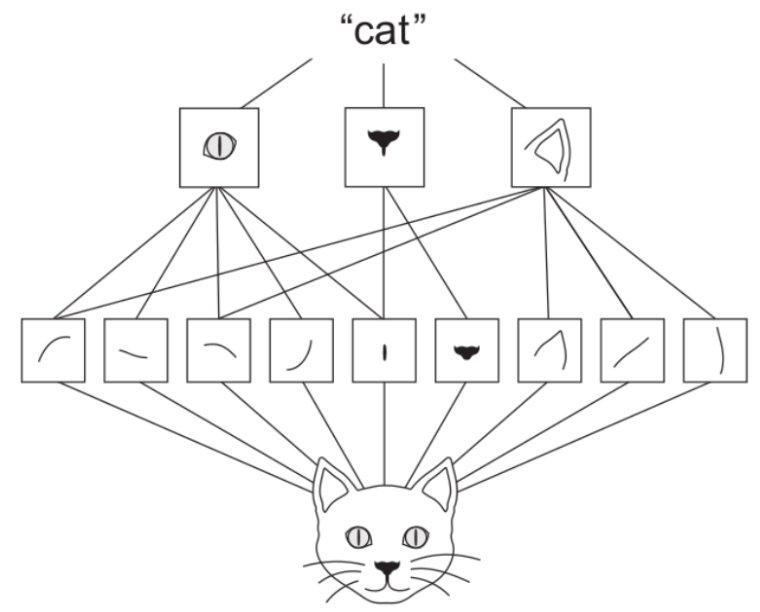
\includegraphics[width=\linewidth]{img/hierarchical_cat.png}
        \caption{Different layers help break down feature detection and selection as hierarchies.}
    \end{subfigure}
    \hfill % optional; add some horizontal spacing
    \begin{subfigure}[b]{0.45\linewidth}
        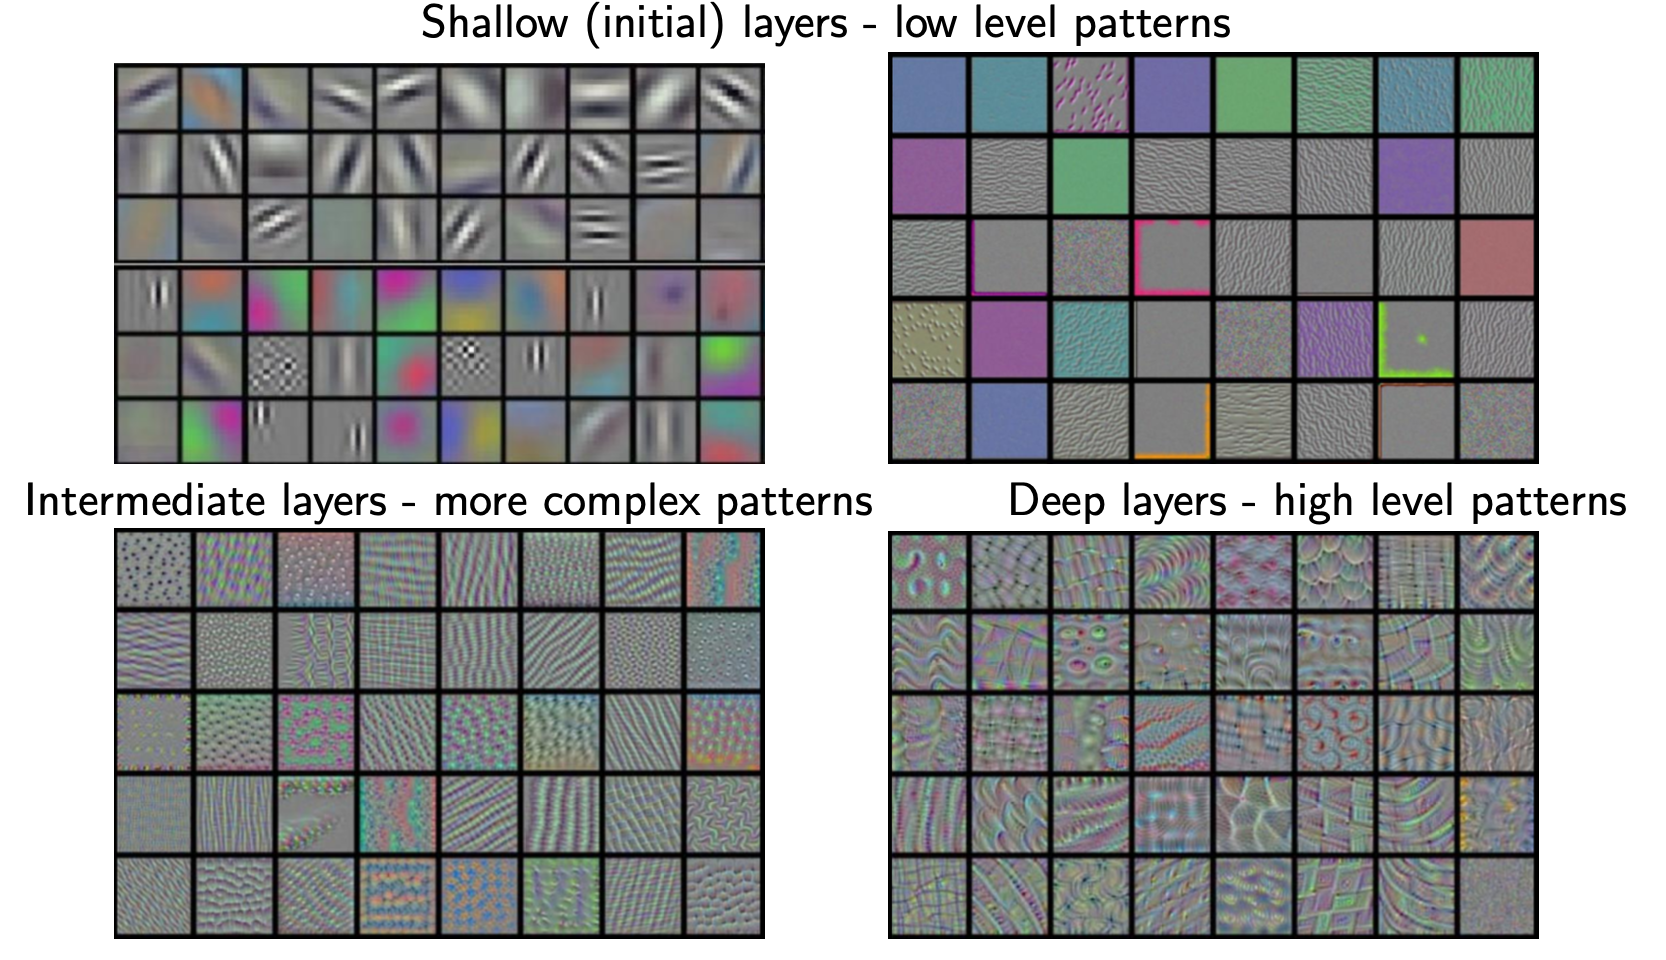
\includegraphics[width=\linewidth]{img/shallow_deep.png}
        \caption{A comparison between shallow and deep networks in terms of feature representation.}
    \end{subfigure}
    \caption{Visualization of hierarchical feature detection in CNNs and the impact of network depth.}
\end{figure}

\end{itemize}

\subsection{CNN Layer Parameters}

The functioning of a CNN is defined by its layer parameters, which dictate how the filters are applied to the input data.

\begin{figure}[H]
    \centering
    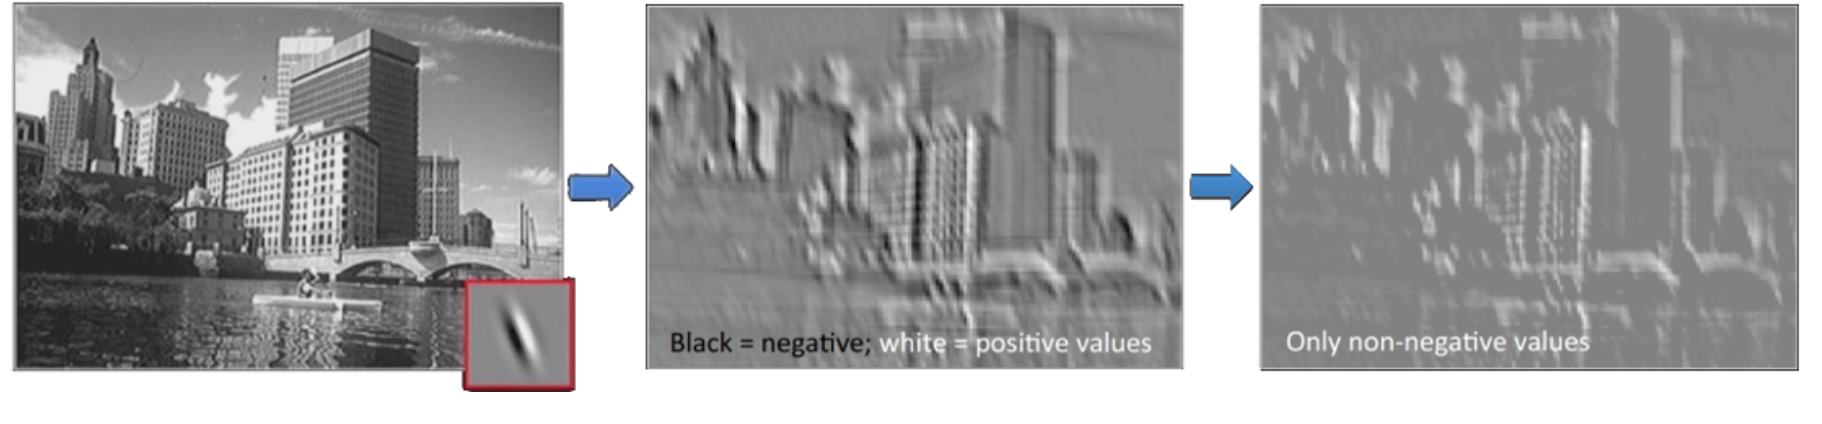
\includegraphics[width=0.75\linewidth]{img/filter_example.png}
    \caption{Filter output and ReLU example}
    
\end{figure}

\begin{itemize}
    \item \textbf{Input:} The input to a convolutional layer is a 3D volume of size \( H_i \times W_i \times D_i \), where \( H_i \) is the height, \( W_i \) is the width, and \( D_i \) is the depth.
    \item \textbf{Parameters:}
    \begin{itemize}
        \item Number of filters \( K \),
        \item Spatial extent of the filter \( F \),
        \item Stride \( S \),
        \item Zero-padding \( P \).
    \end{itemize}
    \item \textbf{Output:} The output is also a 3D volume with dimensions \( H_o \times W_o \times D_o \), given by:
    \begin{itemize}
        \item \( W_o = \frac{W_i - F + 2P}{S} + 1 \),
        \item \( H_o = \frac{H_i - F + 2P}{S} + 1 \),
       
        \item \( D_o = K \).
    \end{itemize}
    \item With \textbf{parameter sharing}, each filter has \( F \cdot F \cdot D_i \) weights, resulting in a total of \( F \cdot F \cdot D_i \cdot K \) weights and \( K \) biases for the layer.
    \item \textbf{Common Settings:} Typically, filters have sizes like \( F \in \{ 2,3,4 \ldots 15\} \), with stride \( S = 1 \) or \( 2 \) and padding \( P  = 0\). Padding can be modified if the post-convolution image needs a different resolution.
    \item In the \textbf{output volume}, the \( d \)-th depth slice (size \( W_o \times H_o \)) corresponds to the activations of the \( d \)-th filter applied at every position of the input, taking stride \( S \) into account and adding the \( d \)-th bias.
\end{itemize}


\section{Pooling Methods}

The pooling layer performs non-linear downsampling via a sliding window across the feature map.It aggregates information from the feature maps obtained from the convolutional layers, and reduces their spatial dimensions while retaining the most important information.\\

A pooling function replaces the output of the network at a certain location with a summary statistic of the nearby outputs– it discards information in the process. For instance, max pooling returns the maximum output within a local region of inputs.\\

This helps reduce the dimensions of data. Common pooling functions include max pooling and average pooling.

\begin{itemize}
    \item \textbf{Max Pooling:} Typically involves \( 2 \times 2 \) filters with a stride of 2, discarding 75\% of the activations. This downsampling reduces each spatial dimension by half, preserving the depth dimension.
    \item \textbf{Average Pooling and L2-Norm Pooling:} These are alternative pooling methods that compute the average and L2 norm of the pooling region, respectively.
\end{itemize}



\begin{figure}[H]
    \centering
    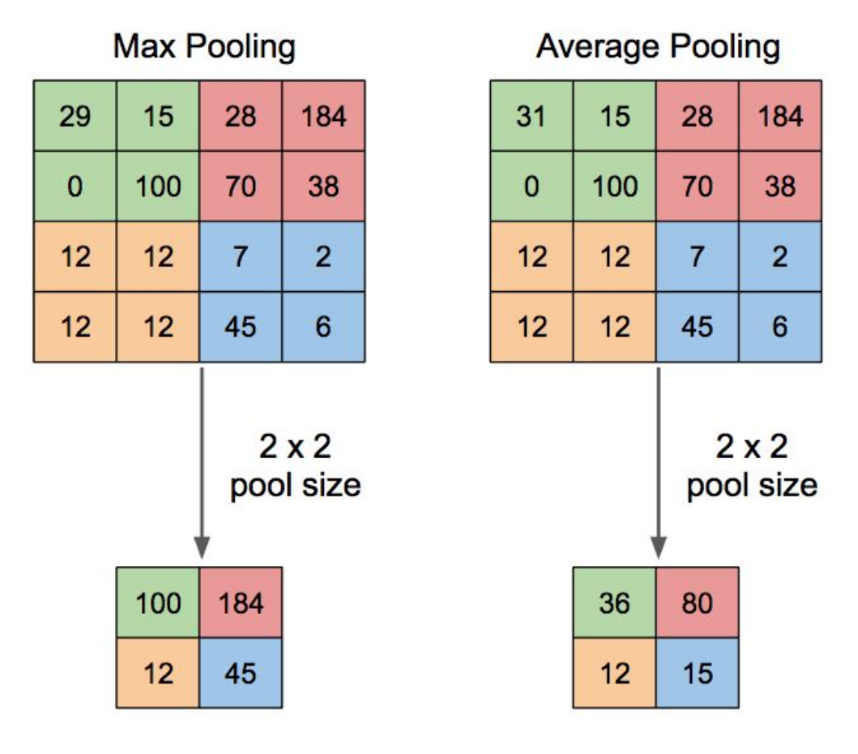
\includegraphics[width=0.4\linewidth]{img/pooling.png}
    
    
\end{figure}

\subsection{Mathematical Description}

Consider a feature map represented by \( A \) where the pooling operation is applied. For a \( 2 \times 2 \) pooling region with stride 2, the max pooling operation can be described as:

\[
Z_{ij} = \max(A_{2i:2i+1, 2j:2j+1})
\]

and for average pooling:

\[
Z_{ij} = \frac{1}{4} \sum_{m=2i}^{2i+1} \sum_{n=2j}^{2j+1} A_{mn}
\]

where \( Z \) is the resulting feature map after pooling, and \( A_{mn} \) denotes the activation in the \( m \)-th row and \( n \)-th column of the feature map \( A \).



The pooling layer operates on the feature maps to perform downsampling, effectively reducing the spatial dimensions while preserving the depth.

\subsubsection{Input and Output Dimensions}

Given an input volume of size \( H_i \times W_i \times D_i \), the output volume \( H_o \times W_o \times D_o \) after the pooling operation is determined by:

\begin{itemize}
    \item \textbf{Spatial Extent \( F \)}: The size of the filter, typically \( F \in \{2, \ldots, 4\} \).
    \item \textbf{Stride \( S \)}: The step size with which the filter moves across the input volume, commonly \( S = 2 \).
    \item \textbf{Padding \( P \)}: Usually set to 0 in pooling layers.
    \item The output dimensions are calculated as:
    \begin{align*}
        W_o &= \frac{W_i - F}{S} + 1, \\
        H_o &= \frac{H_i - F}{S} + 1, \\
        D_o &= D_i.
    \end{align*}
    \item This results in a reduction of the spatial dimensions of the input, with the depth remaining unchanged.
\end{itemize}

\subsubsection{Characteristics of Pooling Layers}


\begin{figure}[H]
    \centering
    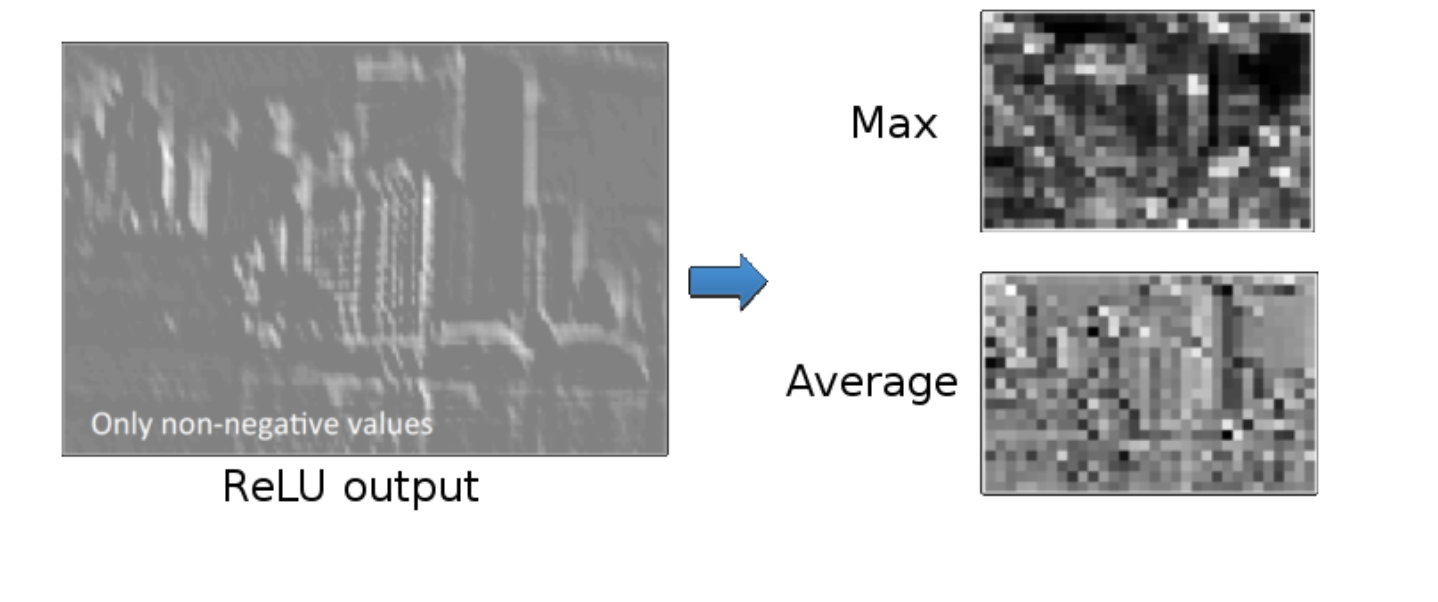
\includegraphics[width=0.5\linewidth]{img/max_avg_pool.png}
    
    
\end{figure}

\subsection{Properties of Pooling Layers}

\begin{itemize}
    \item \textbf{Dimensionality Reduction:} Pooling layers decrease the height and width of the input volume, which reduces the computational load for the subsequent layers.
    \item \textbf{Translational Invariance:} Pooling operations help the network to achieve translational invariance, meaning that shifting the input by a small amount will not change the output of the pooling layer significantly. This makes the CNN less sensitive to the exact spatial locations of features within the input volume.
    \item \textbf{Reduced Sensitivity:} By downsampling, the network becomes less sensitive to the exact location of features in the input space, which contributes to the generalisation capabilities of the network.
    \item \textbf{Efficiency:} Pooling layers reduce the computational load for subsequent layers by decreasing the number of parameters and computations.
    \item \textbf{No Learnable Parameters:} Unlike convolutional layers, pooling layers do not have weights or biases to learn. The pooling operation is deterministic and based solely on the predefined operation, such as max or average pooling.
    \item \textbf{Zero Padding:} Pooling layers typically do not use zero-padding as their primary goal is to reduce dimensionality rather than preserve it.
    \item \textbf{Handling of Varying Input Sizes:} The down-sampling nature of pooling allows CNNs to handle inputs of varying sizes effectively.
\end{itemize}

\subsection{Gradient Propagation}

During backpropagation, the gradient is only passed through the locations that contributed to the maximum in the case of max pooling:

\[
\frac{\partial Z_{ij}}{\partial A_{mn}} = 
\begin{cases} 
1 & \text{if } A_{mn} \text{ is the max value} \\
0 & \text{otherwise}
\end{cases}
\]

For average pooling, the gradient is distributed equally among all the elements of the pooling region.


\section{Fully Connected Layer in CNNs}

The Fully Connected (FC) layer, often found at the end of Convolutional Neural Networks, performs classification tasks by synthesising the features extracted by previous layers to form the final output.

\subsection*{Characteristics of the Fully Connected Layer}

\begin{itemize}
    \item It operates on a flattened input where all the spatial information is converted into a single vector of neurons.
    \item Each neuron in a fully connected layer is connected to all activations in the previous layer, resulting 
    \item It is the final learning phase that maps the extracted features to the desired outputs.
    \item The layer's adaptability makes it suitable for both classification and encoding tasks.
\end{itemize}

\subsection*{Mathematical Formalism}

The operations within a Fully Connected layer can be described mathematically as follows:\\

Given an input feature map $F \in \mathbb{R}^{h \times w \times d}$, where $h$, $w$, and $d$ represent height, width, and depth respectively, the feature map is flattened into a vector $v \in \mathbb{R}^{hwd}$.\\

This vector is then transformed by the FC layer using a weight matrix $W \in \mathbb{R}^{n \times hwd}$ and a bias vector $b \in \mathbb{R}^{n}$, with $n$ being the number of neurons in the FC layer. The output $o \in \mathbb{R}^{n}$ of the FC layer is given by:

\begin{equation}
o = \sigma(Wv + b)
\end{equation}

where $\sigma$ denotes the activation function, which can be a sigmoid, softmax, or any other non-linear function. In the context of classification, the softmax function is commonly used to convert the output into probability distributions:

\begin{equation}
\text{Softmax}(o_i) = \frac{e^{o_i}}{\sum_{j=1}^{n} e^{o_j}} \quad \text{for } i=1,2,\ldots,n
\end{equation}

\subsection*{Sequence in CNNs}

The typical sequence of operations in a CNN before reaching the FC layer is:

\begin{enumerate}
\item \textbf{Convolution:} Extracts features by applying filters to the input.
\item \textbf{Pooling:} Reduces the spatial size of the representation, decreasing the number of parameters and computation in the network.
\item \textbf{Flattening:} Transforms the 2D feature maps into a 1D feature vector.
\item \textbf{Fully Connected Layer:} Utilises the flattened vector for classification or regression tasks.
\end{enumerate}

\begin{figure}
    \centering
    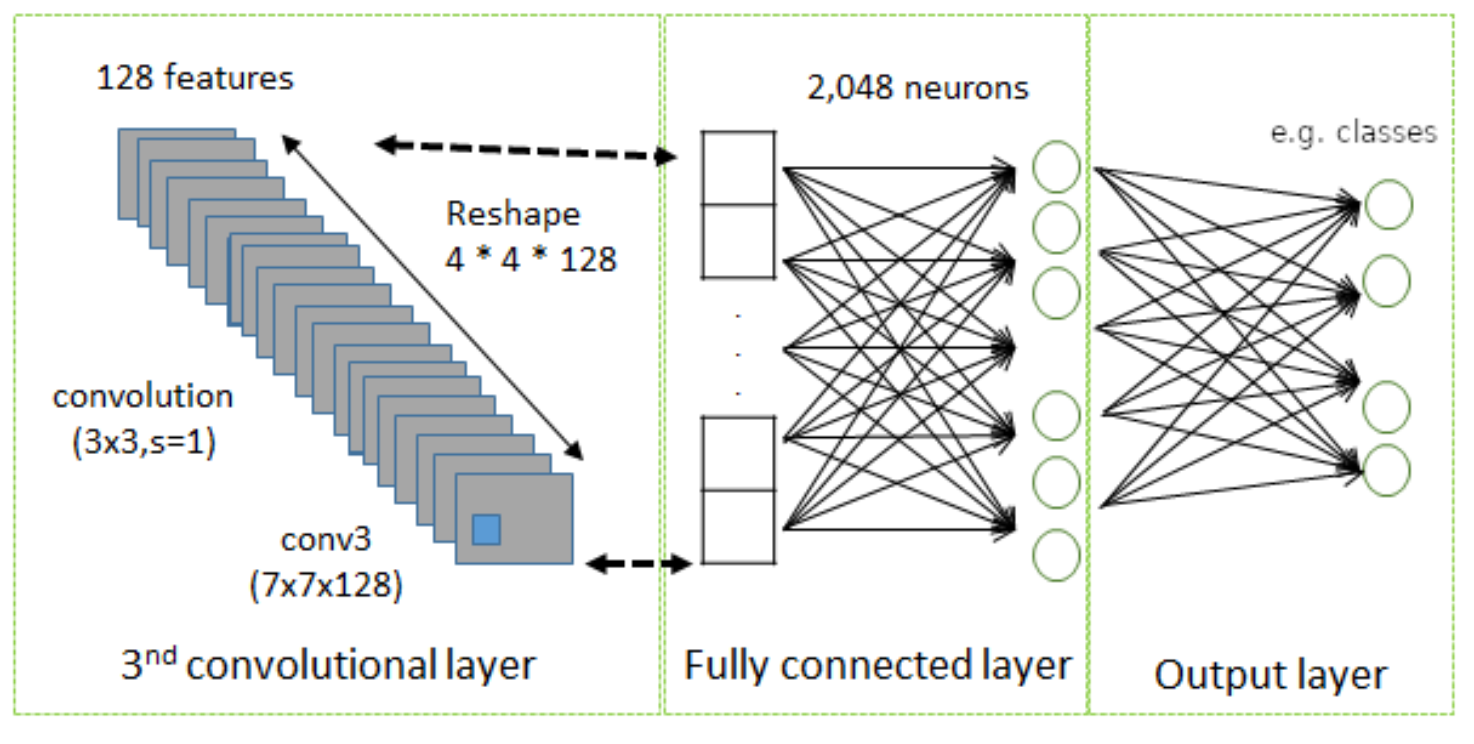
\includegraphics[width=0.75\linewidth]{img/FC.png}
    \caption{Visualisation of the FC Layer} 
\end{figure}

\section{Loss Layer}
\begin{itemize}
    \item The loss layer is required for training the network.
    \item Input: It takes in network predictions and the ground truth, which are samples of the target function.
    \item Output: the prediction error as a scalar
    \item The Loss function can be set depending on the task and data. 
    \item For classification, the softmax (sigmoid) activation function is used followed by cross-entropy loss.
    \item For regression, L1, L2, and Smooth L2 losses are used.
\end{itemize}

\subsection*{Loss Layer for Binary Classification}

Binary classification in CNNs can be thought of as a decision-making process, where the network learns to differentiate between two distinct classes (e.g., 'dog' vs 'no dog'). The sigmoid function squashes the output of the linear combination of inputs and weights into a range between 0 and 1, giving us a probability score. The cross-entropy loss then quantifies the difference between the predicted probability and the actual class. A lower loss indicates better model performance, implying that the predicted probability is closer to the actual class label.


\begin{figure}[H]
    \centering
    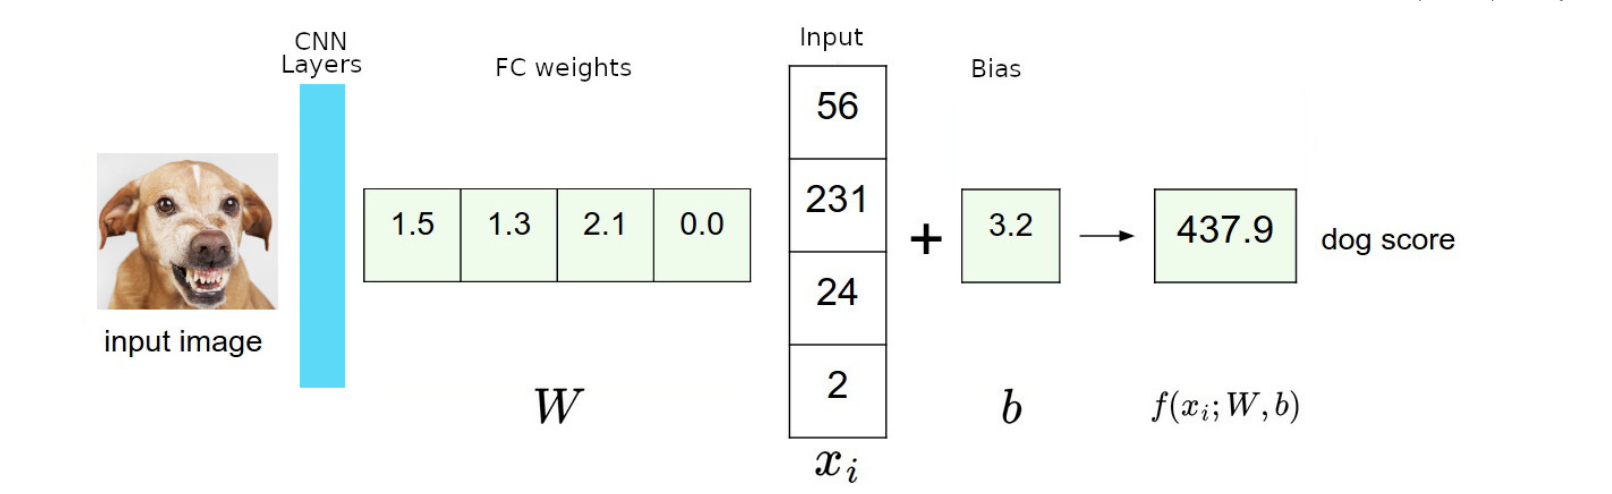
\includegraphics[width=0.6\linewidth]{img/dogloss.png}
    \caption{Graphical representation of Log Loss when the true label is 1.}
\end{figure}


\begin{itemize}
    \item Given a ground truth label \( y \) and a network prediction \( \hat{y} \), where \( y \in \{0,1\} \) and \( \hat{y} \) is the sigmoid activation function applied to the linear combination of inputs and weights:
    \[ \hat{y} = \frac{e^{W^Tx+b}}{e^{W^Tx+b}+1} \]
    \item This formulation allows \( \hat{y} \) to be interpreted as the probability of the input being classified as class 1 (for example, detecting if an image contains a dog).
    
    \item The \textbf{Cross-entropy loss function} \( \mathcal{L} \) is defined as:
    \[ \mathcal{L} = -y \log(\hat{y}) - (1-y) \log(1-\hat{y}) \]
    This function penalises the deviation of \( \hat{y} \) from the true label \( y \). It is particularly sensitive to confident but incorrect predictions, which is desirable in a loss function.
\end{itemize}



For an input image classified with a high confidence (\( \hat{y} \approx 1 \)), and the true label being 1 (indicating presence of a dog), the loss is close to 0 as seen in the function:
\[ \mathcal{L} = -1 \log(1) + (1-1) \log(1 - \hat{y}) = 0 \]

Note that \( \hat{y} \) as a probability is never exactly 0 or 1 but always in between, reflecting a degree of uncertainty.

\subsection*{Loss Layer for Multiclass Classification}

Multiclass classification is akin to a voting system where each class competes for the highest probability score. The Softmax function acts like a normaliser, converting raw scores (logits) into probabilities that sum up to one. The cross-entropy loss then measures how well the predicted probability distribution aligns with the actual distribution (the ground truth). 



\begin{itemize}
    \item For a multi-label ground truth vector \( \mathbf{y} \) and a prediction vector \( \hat{\mathbf{y}} \in \mathbb{R}^K \), where \( K \) is the number of classes, the model uses the \textbf{Softmax} function for the prediction:
    \[ \hat{y}_k = \frac{e^{W_k^T\mathbf{x}+b}}{\sum_{i}e^{W_i^T\mathbf{x}+b}} \]
    \item The \textbf{Categorical (multiclass) cross entropy error} \( \mathcal{L} \) for each class \( k \) is computed as:
    \[ \mathcal{L}_k = -y_k \log(\hat{y}_k) \]
    This error is summed or averaged over all classes to provide a total loss for a single prediction.
    
    \item It is often noted that this method is \textbf{superior to classification error or Mean Squared Error (MSE)}:
    \begin{itemize}
        \item \textit Classification error ignores the confidence of the predictions.
        \item MSE places too much emphasis on incorrect outputs, which can lead to poor performance in classification tasks.
    \end{itemize}
\end{itemize}


\begin{figure}[H]
    \centering
    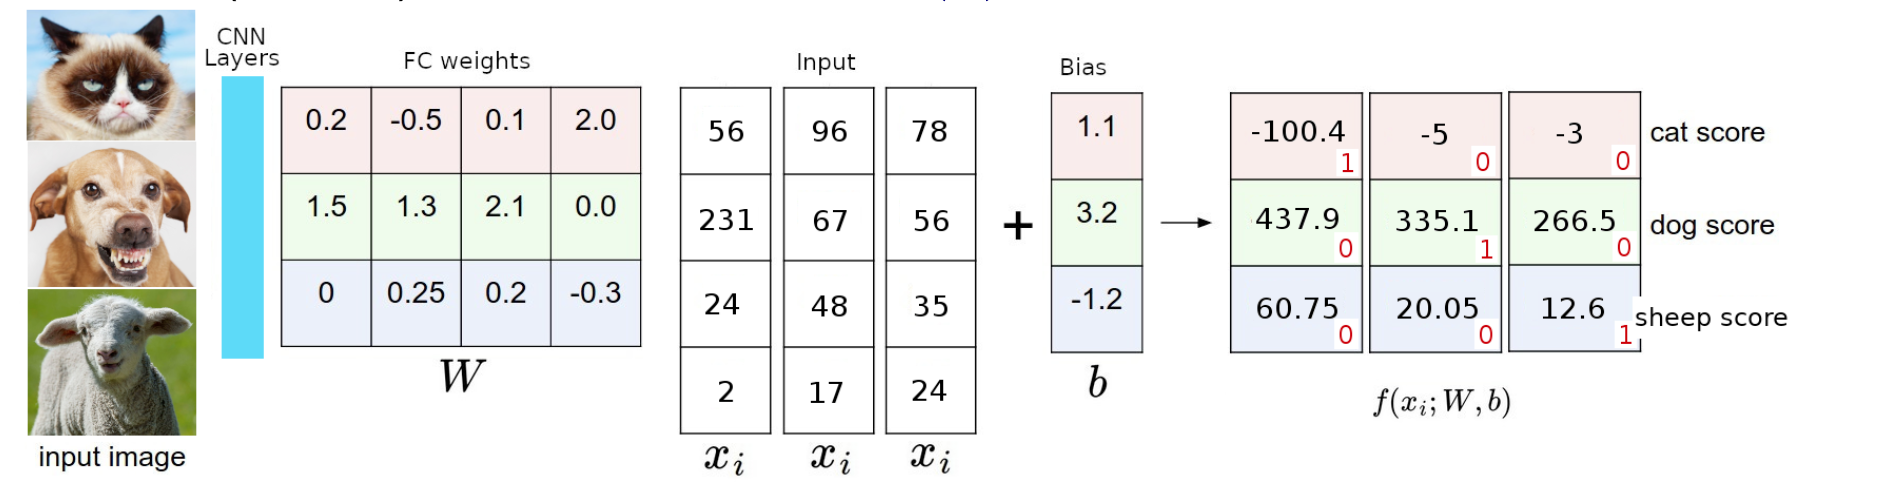
\includegraphics[width=0.85\linewidth]{img/animals.png}
    \caption{Diagram of a categorical (multiclass) loss layer. Note that one image is sent as an input.}
    
\end{figure}

\subsubsection*{Average Cross Entropy Loss Calculation Example}
For an example with three classes, represented as `cat`, `dog`, and `sheep`, the average cross entropy (ACE) loss \( \mathcal{L} \) would be calculated for a single instance as:
\[ \mathcal{L} = \frac{1}{3} \left( -y_{1} \log(\hat{y}_{1}) + -y_{2} \log(\hat{y}_{2}) + -y_{3} \log(\hat{y}_{3}) \right) \]

So the cat score \(\hat{y}_{1,1}=\frac{e^{-100.4}}{e^{-100.4}+e^{437.9}+e^{60.75}}\)

\subsubsection*{Hinge loss comparison}

\[\mathcal{L}=\sum_{j\neq k}\max(0,\hat{y}_j-\hat{y}_k+1)\]

The hinge loss calculation is the sum of the differences between the score for the non-correct classes and the score for the correct class (plus the margin), but only when those differences are positive.

This is typically used with Support Vector Machine (SVM) models.



\begin{figure}[H]
    \centering
    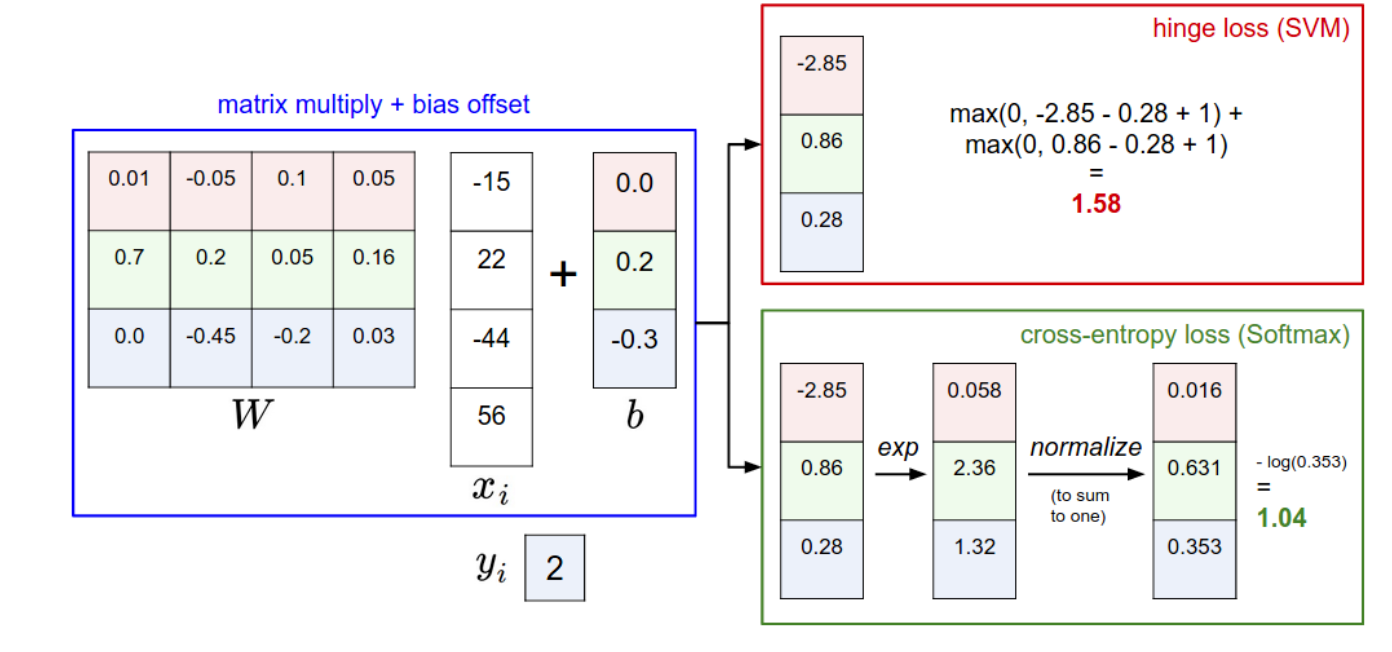
\includegraphics[width=1\linewidth]{img/hinge_softmax.png}
    \caption{Comparison of layers for of Cross Entropy Loss vs Hinge Loss}
    \label{fig:enter-label}
\end{figure}

\section{Loss Layer for Regression}

In regression tasks within machine learning, the goal is to predict continuous values, and the loss layer is responsible for measuring the discrepancy between the predicted values \( \hat{y} \) and the actual ground truth values \( y \).

\begin{itemize}
    \item The \textbf{L2 Loss} or \textbf{Mean Squared Error (MSE)} is the square of the Euclidean distance between the network's prediction and the true value:
    \[ \mathcal{L}_2 = \lVert wx + b - y \rVert^2 = (wx + b - y)^2 \]
    \[ \text{MSE} = \frac{1}{N} \sum_{i=1}^{N} \mathcal{L}_2(i) \]
    where \( N \) is the number of samples.

    \item The \textbf{L1 Loss} or \textbf{Mean Absolute Error (MAE)} measures the absolute difference:
    \[ \mathcal{L}_1 = \lvert wx + b - y \rvert \]
    \[ \text{MAE} = \frac{1}{N} \sum_{i=1}^{N} \mathcal{L}_1(i) \]

    \item \textbf{Smooth L1 Loss} (also known as Huber loss) is a combination of L1 and L2 losses:
    \[ \mathcal{L}_{\text{smooth}} = \begin{cases} 
    0.5 \times \mathcal{L}_2, & \text{for } \mathcal{L}_1 < 0.5 \\
    \mathcal{L}_1 - 0.5, & \text{otherwise}
    \end{cases} \]
    This loss is less sensitive to outliers than L2 loss.
\end{itemize}

The graph on the slide provides a visual comparison of these loss functions. The L2 loss increases quadratically and is more sensitive to larger errors, while the L1 loss grows linearly. The Smooth L1 Loss combines these two behaviours: it is quadratic for small errors and linear for large errors, which makes it robust to outliers.

\begin{figure}[H]
\centering
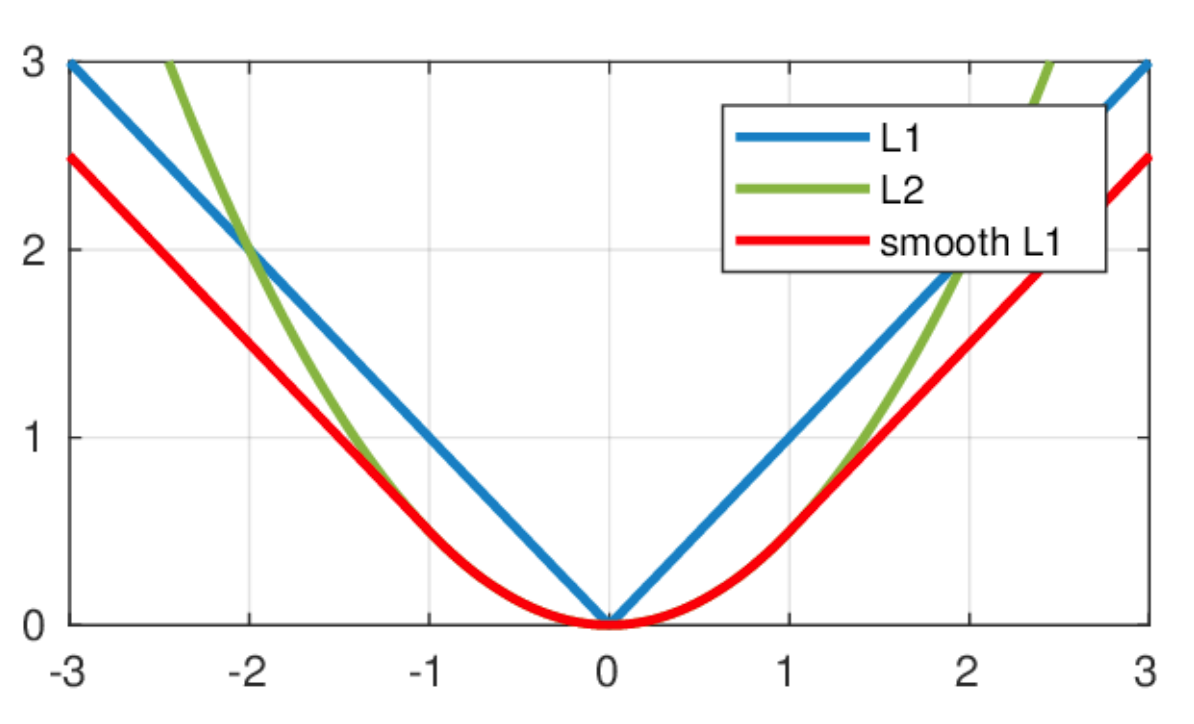
\includegraphics[width=0.5\textwidth]{img/l1_l2.png}
\caption{Comparative graph of L1, L2, and Smooth L1 Loss functions.}
\end{figure}

In practice, the choice of loss function can significantly affect the regression model's performance, particularly in terms of sensitivity to outliers in the training data.
\begin{figure}[H]
    \centering
    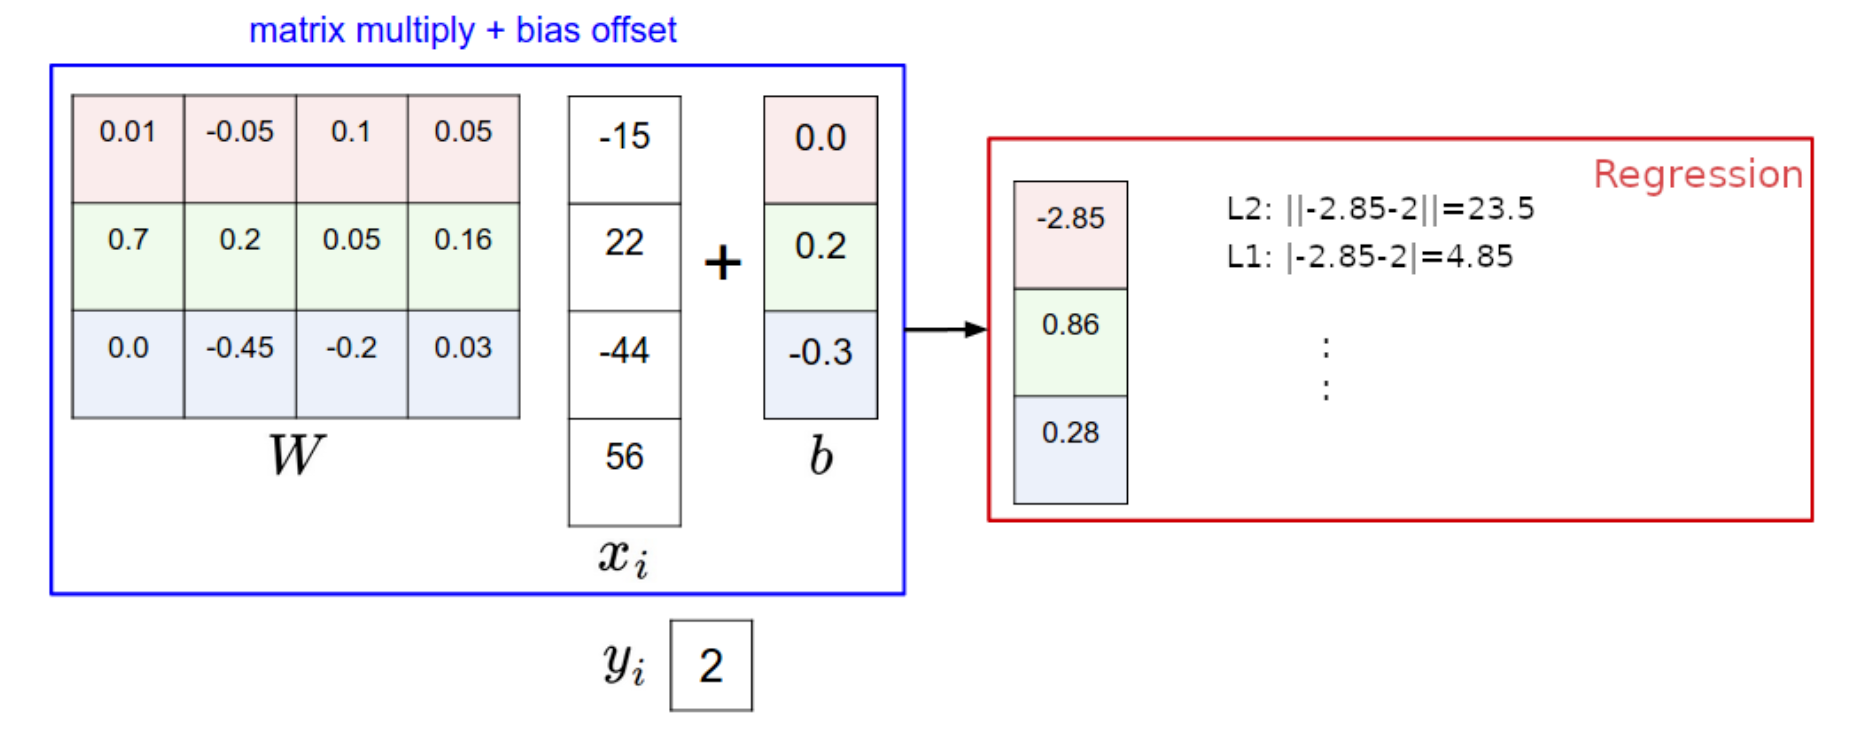
\includegraphics[width=1\linewidth]{img/losslayer-regression.png}
    \caption{Diagram of a categorical (multiclass) regression loss layer }
\end{figure}


\section{Practical Hints for CNNs}

\subsection*{Number of Filters}
\begin{itemize}
    \item The number of filters in a CNN directly influences the network's capacity and its ability to capture features from the input data.
    \item This number should be balanced with the complexity of the task and the volume of available training data.
    \item Computing activations with convolutional operations is more computationally expensive than in Multilayer Perceptrons (MLPs), even though the size of the neuron is smaller.
    \item Typically, initial layers have fewer filters compared to deeper layers. This reflects the progression from capturing basic features to more complex ones.
    \item Adjusting the number of filters can balance the computational load across the network and maintain a consistent level of feature representation at each layer.
\end{itemize}

\subsection*{Filter Shape}
\begin{itemize}
    \item The dimensions of the filters depend on the type of input data and the abstractions that the network needs to learn.
    \item Large filters (e.g., 11x11) are often used in the first layers to capture broad features, while smaller filters (e.g., 5x5) are used in deeper layers for finer details.
\end{itemize}

\subsection*{Pooling}
\begin{itemize}
    \item Pooling layers reduce the spatial dimensions of the feature maps. Typical configurations include 2x2 or no max-pooling.
    \item The trend in deep learning is moving towards using smaller filters and deeper architectures, sometimes foregoing pooling layers to preserve information.
    \item For inputs with large spatial dimensions, larger pooling (e.g., 4x4) might be used, but there is a risk of losing too much detail.
\end{itemize}

\subsection*{Loss Functions}
\begin{itemize}
    \item For classification tasks, the Softmax function is typically used in conjunction with a cross-entropy loss.
    \item In regression tasks, L2 (Mean Squared Error) or Smooth L1 (Huber Loss) are common choices for loss functions.
\end{itemize}

\subsection*{Typical Sequence of Layers in Shallow Networks}
\begin{itemize}
    \item A common architecture sequence for shallow networks is:
    \begin{verbatim}
        INPUT → [CONV → Norm → RELU → POOL] (x2) → FC → RELU → FC → OUTPUT
    \end{verbatim}
    \item Another variant might be:
    \begin{verbatim}
        INPUT → [CONV → RELU → CONV → RELU → POOL] (x3) → [FC → RELU] (x2) → FC → OUTPUT
    \end{verbatim}
\end{itemize}

    
    
